\section{The C-{}- language}
In this section we present the implementation of a small imperative language called C-{}-. Note that, although the name might suggest this, we do not claim any resemblance with the C programming language, as it lacks several features such as pointer arithmetic, arrays, and functions.

C-{}- allows the use of four built-in values: integer, strings, booleans, and floating-point numbers in double precision. The memory is represented using a dictionary that pairs variable names with their value. In what follows we omit the details of the lookup of entries in the dictionary for brevity. Suffice to say that the meta-program makes use of the \texttt{ImmutableDictionary} data structure available in .NET. Also note that C-{}- defines scopes for variables, so that if a variable is declared inside the scope of a code block in a control structure, that is usable only within the scope itself.

The core of the meta-program is made of the evaluation of both expressions and statements. We proceed below to present the details of both kinds of evaluation.

\subsection{Expression Evaluation}
As explained above C-{}- supports boolean, string, integer, and floating-point values. These are represented through the following meta-data structures in the meta-program.

\begin{lstlisting}
Data "$i" -> <<int>> : Value Priority 300
Data "$d" -> <<double>> : Value Priority 300
Data "$s" -> <<string>> : Value Priority 300
Data "$b" -> <<bool>> : Value Priority 300
\end{lstlisting}

\noindent
Note that we are using the .NET data types to represent the actual values stored in the meta-data structures.

\subsection{Statement Evaluation}

\section{Casanova 2.5 in Metacasanova}
In this section we will briefly introduce the Casanova language, a domain specific language for games. We then show a re-implementation, which we call Casanova 2, of the Casanova 2 language hard-coded compiler as an example of use of Metacasanova.


%expand with the full implementation of Casanova 2
\subsection{The Casanova language}
Casanova 2.5 is a language oriented to video game development which is based on Casanova 2 \cite{CASANOVA2_PAPER}. A program in Casanova is a tree of \textit{entities}, where the root is marked in a special way and called \textit{world}. Each entity is similar to a \textit{class} in an object-oriented programming language: it has a constructor and some fields. The fields do not have access modifiers because they are not directly modifiable from the code except with a specific statement. Each entity also contains a list of \textit{rules}, that are methods that are ticked in order with a specific refresh rate called \texttt{dt}. Each rule takes as input four elements: \texttt{dt}, \texttt{this}, which is a reference to the current entity, \texttt{world} that is a reference to the world entity, and a subset of entity fields called \textit{domain}. A rule can only modify the fields contained in the domain. The rules can be paused for a certain amount of seconds or until a condition is met by using the \texttt{wait} statement. It is possible to modify the values of the fields in the domain by using the \texttt{yield} statement which takes as input a tuple of values to assign to the fields. When the \texttt{yield} statement is executed the rule is paused until the next frame. Also the body of control structures (\texttt{if-then-else}, \texttt{while}, \texttt{for}) is interruptible. In the following section we show the implementation of Casanova 2.5 in Metacasanova.

\subsection{Casanova 2.5}
The memory in Casanova 2.5 is represented using three maps, where the key is the variable/field name, and the value is the value stored in the variable/field. The first dictionary represents the global memory (the fields of the \texttt{world} entity or \textit{Game State}), the second dictionary represents the current entity fields, and the third the variable bindings local to each rule.

The core of the entity update is the \texttt{tick} function. This function evaluates in order each rule in the entity by calling the \texttt{evalRule} function. This function executes the body of the rule and returns a result depending on the set of statements that has been evaluated. This result is used by \texttt{tick} to update the memory and rebuild the rule body to be evaluated at the next frame. The result of \texttt{tick} is a \texttt{State} containing the rules updated so far, and the updated entity and global fields. Since a rule must be restarted after the whole body has been evaluated, we need to store a list containing the original rules, which will be restored when evaluation returns \texttt{Done} (see below). At each step the function recursively calls itself by passing the remaining part of original rules (the rules which body was not altered by the evaluation of the statements) and modified rules (which body has been altered by the evaluation of the statements) to be evaluated. The function stops when all the rules have been evaluated, and this happens when both the original and the modified rule lists are empty.

Interruption is achieved by using \textit{Continuation passing style}: the execution of a sequence of statements is seen as a sequence of steps that returns the result of the execution and the remaining code to be executed. Every time a statement is executed we rebuild a new rule whose body contains the continuation which will be evaluated next. 

\begin{comment}
For example, consider the following rule:

\begin{lstlisting}
rule X,Y =
while X > 0 do
wait 1.0f
yield X - 1,Y + 1
\end{lstlisting}

The code is executed atomically until the \texttt{wait} statement (assuming that the \texttt{while} condition is true). At that point we rebuild a new rule containing the code to execute at the next iteration:

\begin{lstlisting}
rule X,Y =
wait (1.0f - dt)
yield X - 1, Y + 1
while X > 0 do
wait 1.0f
yield X - 1,Y + 1
\end{lstlisting}
Note that the \texttt{while} is placed at the end of the continuation because it must be re-evaluated after the first iteration is complete, and that we have decreased the waiting time by \texttt{dt} (the time elapsed between one frame and the previous one).
\end{comment}

The possible results returned by the \texttt{tick} function are the following: (\textit{i}) \texttt{Suspend} contains a \texttt{wait} statement with the updated timer, the continuation, and a data structure called \texttt{Context} which contains the updated local variables, the entity fields, and the global fields. The function rebuilds a rule which body is the sequence of statements contained by the \texttt{Suspend} data structure. (\textit{ii}) \texttt{Resume} is returned when the timer must resume after the last waited frame. In order not to skip a frame we must still re-evaluate the rule at the next frame and not immediately. In this case the argument of \texttt{Resume} is only the remaining statements to be executed. (\textit{iii}) \texttt{Yield} stops evaluation for one frame. We use the continuation to rebuild the rule body. Memory is updated by \texttt{evalRule}. (\textit{iv}) \texttt{Done} stops the evaluation for one frame and rebuilds the original rule body by taking it from the original rules list.

For brevity we write only the code for \texttt{Suspend}. A full implementation can be found at \cite{CASANOVA_SOURCE_CODE}. You can see a schematic representation of the tick function in Figure \ref{fig:tick}.

\begin{lstlisting}
evalRule (rule dom body k locals delta) fields globals => Suspend (s;cont) (Context newLocals newFields newGlobals)
r := rule dom s cont newLocals dt
tick originals rs newFields newGlobals dt => State updatedRules updatedFields updatedGlobals
st := State (r::updatedRules) updatedFields updatedGlobals
------------------------------------------------------
tick (original::originals) ((rule dom body k locals delta)::rs) fields globals dt => st
\end{lstlisting}


\begin{figure}
	\centering
	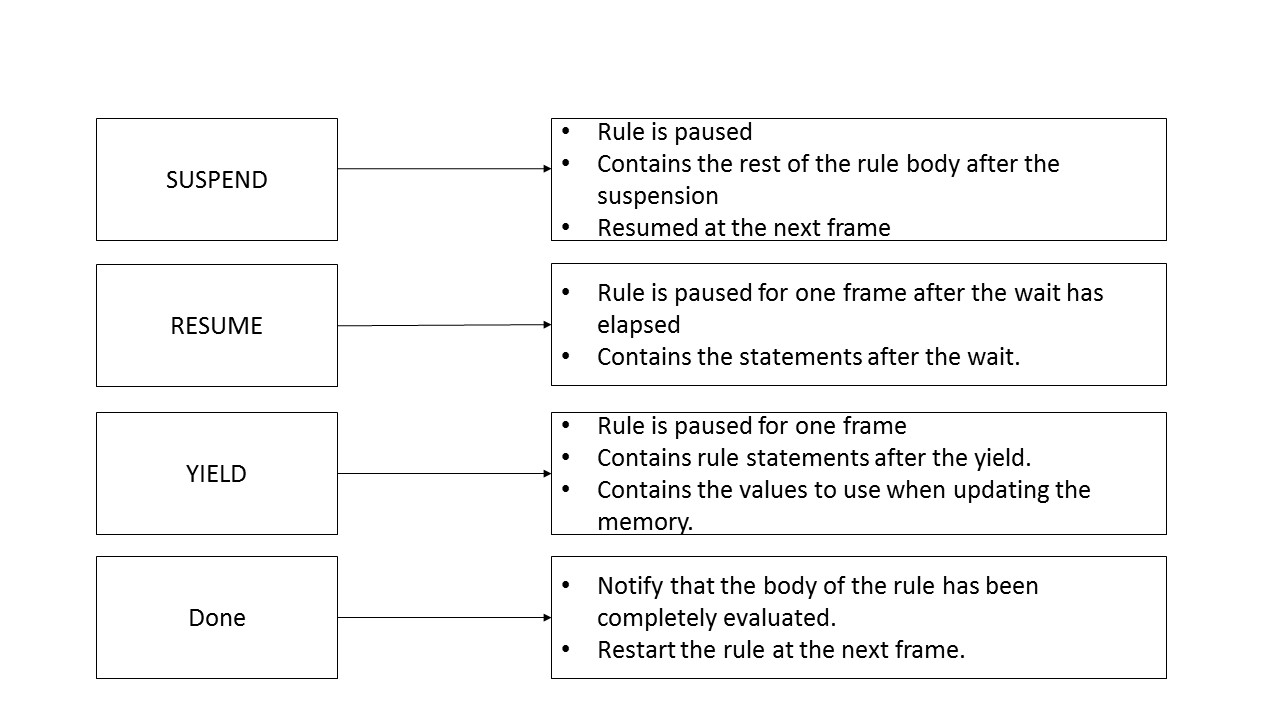
\includegraphics[scale = 0.25]{Figures/tick2}
	\caption{Casanova 2.5 rule evaluation}
	\label{fig:tick}
\end{figure}

The function \texttt{evalRule} calls \texttt{evalStatement} to evaluate the first statement in the body of the rule passed as argument. The result of the evaluation of the statement is processed in the following way: (\textit{i}) if the result is \texttt{Done}, \texttt{Suspend} or \texttt{Resume} then it is just returned to the caller function. We omit the code for this case, since it is trivial; (\textit{ii}) if the result is \texttt{Atomic} it means that the evaluated statement was uninterruptible and the remaining statements of the rule must be re-evaluated immediately; (\textit{iii}) if the result is \texttt{Yield} then the fields in the domain are updated recursively in order and then the updated memory is encapsulated in the \texttt{Yield} data structure and passed to the caller function.

\vspace{0.1cm}
\begin{lstlisting}
evalStatement b k ctxt dt => Atomic z c    
evalRule (rule dom z nop c dt) => res
-------------------------------
evalRule (rule dom b k ctxt dt)  => res
\end{lstlisting}

\begin{lstlisting}
evalStatement b k (Context locals fields globals) dt => Yield ks values context
updateFields dom values context  => updatedContext
--------------------------------------------------------
evalRule (rule dom b k locals dt) fields globals => Yield ks values updatedContex
\end{lstlisting}

Note that, in case of a rule containing only atomic statements, we will eventually return \texttt{Done} after having recursively called \texttt{evalStatement} for all the statements, and the rule will be paused for one frame.

\begin{comment}
\begin{figure}
\centering
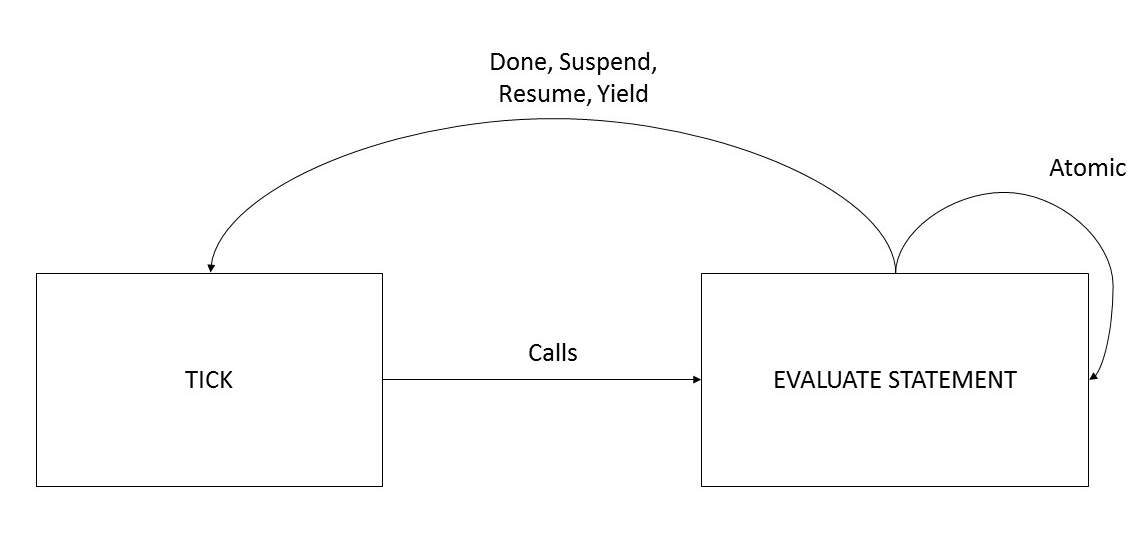
\includegraphics[scale=0.15]{Pictures/statement_evaluation}
\caption{Statement evaluation}
\label{fig:statement_evaluation}
\end{figure}
\end{comment}

\noindent
The \texttt{evalStatement} function is used both to evaluate a single statement and a sequence of statements. When evaluating a sequence of statements, the first one is extracted. A continuation is built with the following statement and passed to a recursive call to \texttt{evalStatement} which evaluates the extracted statement. If the existing continuation is non-empty, then it is added before the current continuation. If both the continuation and the body are empty (situation represented by the \texttt{nop} operator) then it means the rule evaluation has been completed and we return \texttt{Done}.

\begin{lstlisting}
a != nop
---------------------                           ----------------------- 
addStmt a b => a;b                              addStmt nop nop => nop   

addStmt b k => cont
evalStatement a cont ctxt dt => res
-------------------------------                 -----------------------------------       
evalStatement (a;b) k ctxt dt => res            evalStatement nop nop ctxt dt => Done ctxt


\end{lstlisting}

\noindent
We will now present, for brevity, only the evaluation of the \texttt{wait} and \texttt{yield} statements. Both the evaluation of the control structures and the variable bindings always return \texttt{Atomic} because they do not, by definition, pause the execution of the rule.

The \texttt{wait} statement has two different evaluations, based on the rules defined in Section \ref{sec:problem_statement}: (\textit{i}) the timer has elapsed: in this case we return \texttt{Resume} which contains the code to execute after the \texttt{wait} statement, or (\textit{ii}) the timer has not elapsed: in this case we return \texttt{Suspend} which contains the \texttt{wait} statement with the updated timer followed by the continuation.


\begin{lstlisting}
<<t <= dt>> == false
----------------------------------
evalStatement (wait t) k ctxt dt => Suspend wait <<t - dt>>;k ctxt

<<t <= dt>> == true
----------------------------------
evalStatement (wait t) k ctxt dt => Resume k ctxt
\end{lstlisting}

\noindent
The \texttt{yield} statement takes as argument a list of expressions whose values are used to update the corresponding fields in the rule domain. The evaluation rule recursively evaluates the expressions and stores them into a list passed as argument of the \texttt{Yield} result. Those arguments are used later by \texttt{evalRule} to update the corresponding fields.

\begin{lstlisting}
eval expr ctxt => v
evalYield exprs ctxt => vs
-------------------------------------------          ----------------------------
evalYield (expr :: exprs) ctxt => v :: vs            evalYield nil ctxt => nil
\end{lstlisting}

In this section we provide an implementation of a patrol script for an entity in a game. The sample is made up of an entity, representing a guard, and a couple of checkpoints. The guard continuously moves between the two checkpoints. We choose this sample because this is a typical behaviour implemented in several games, where the user is able to set up a patrol route for a unit. We show the comparison between the sample implemented in Casanova 2.5 and an equivalent implementation in Python with respect to the running time. We then show a comparison between the hard-coded compiler of Casanova 2.0 and the implementation of Casanova 2.5 in Metacasanova with respect to the code length. 

\begin{comment}
We want to underline that the main goal of this work is \textbf{to ease the process of building a compiler for a DSL for games, thus our main objective is decreasing the code length and complexity necessary to implement a hard-coded compiler for the language}. At the same time we show that the compiled program in Casanova 2.5 \textbf{has performance similar to that of a language used in game development, and thus Casanova 2.5 is usable in a real scenario}.
\end{comment}

\subsection{Chosen languages}
We compared the running time of the sample in metacompiled Casanova with an equivalent implementation in Python. This language was chosen based on its use in game development: Python has been used extensively in several games such as Civlization IV \cite{CIV4} or World in Conflict \cite{WIC} because of the native support for coroutines. We deliberately ignore C++ and C\# implementations, although they are widely used in the industry, because we knew in advance \cite{CASANOVA2_PAPER} that the current version of the code generated by the meta-compiler would not match the high performance of these languages: the main goal of this work is to reduce the effort of writing a compiler for a DSL for games while having acceptable performance.


\subsection{Performance}
The performance results are shown in Table \ref{tab:evaluation}. We see that the generated code has performance on the same order as Python. This is mainly due to the fact that the memory, in the metacompiled implementation of Casanova, is managed through a map, and because of the virtuality of the implemented operators. Each time Casanova accesses a field in an entity this must be looked up into the map. To this we add the complexity of dynamic lookups when we must deal with polymorphic results into the rules. 

From Table \ref{tab:compiler_comparison} we see that the implementation of Casanova 2.0 language in Metacasanova is almost 5 times shorter in terms of lines of code than the previous Casanova implementation in F\#. We believe it is worthy noticing that structures with complex behaviours, such as \textit{wait} or \textit{when}, require hundreds of lines of codes with a standard approach (the code lines to define the behaviour of the structure plus the support code to correctly generate the state machine), while in the meta-compiler we just need tens of lines of codes to implement the same behaviour. Moreover we want to point out that the previous Casanova compiler was written in a functional programming language: these languages tend to be more synthetic than imperative languages, so the difference with the same compiler implemented in languages such as C/C++ might be even greater.

The readability with respect to the hard-coded compiler code is also improved: we managed to implement the behaviour of synchronization and timing primitives almost imitating one to one the formal semantics of the language definition (see the semantics rules in Section \ref{sec:formal_description} and their implementation in Section \ref{sec:casanova3}). In the hard-coded compiler implementation for Casanova 2.0 the semantics are lost in the code for generating finite state machines.

\begin{table}[!h]
	\centering
	\tiny	
	\begin{tabular}{|c|c|c|}
		\hline
		\multicolumn{3}{|c|}{\textbf{Casanova 2.5}} \\
		\hline
		Entity \# & Average update time (ms) & Frame rate \\
		\hline
		100 & 0.00349 & 286.53 \\
		\hline
		250 & 0.00911 & 109.77 \\
		\hline
		500 & 0.01716 & 58.275 \\
		\hline
		750 & 0.02597 & 38.506 \\
		\hline
		1000 & 0.03527 & 28.353 \\
		\hline
		\multicolumn{3}{|c|}{\textbf{Python}} \\
		\hline
		Entity \# & Average update time (ms) & Frame rate \\
		\hline
		100 & 0.00132 & 756.37 \\
		\hline
		250 & 0.00342 & 292.05 \\
		\hline
		500 & 0.00678 & 147.54 \\
		\hline
		750 & 0.01087 & 91.988 \\
		\hline
		1000 & 0.01408 & 71.002 \\
		\hline
	\end{tabular}
	\caption{Patrol sample evaluation}
	\label{tab:evaluation}
\end{table}

\begin{table}[!h]
	\centering
	\tiny
	\begin{tabular}{|c|c|}
		\hline
		\multicolumn{2}{|c|}{\textbf{Casanova 2.5 with Metacasanova}} \\
		\hline
		Module & Code lines \\
		\hline
		Data structures and function definitions & 40 \\
		\hline
		Query Evaluation & 16 \\
		\hline
		While loop & 4 \\
		\hline
		For loop & 5 \\
		\hline
		If-then-else & 4 \\
		\hline
		When & 4 \\
		\hline
		Wait & 6 \\
		\hline
		Yield & 10 \\
		\hline
		Additional rules for Casanova program evaluation & 40 \\
		\hline
		Additional rules for basic expression evaluation & 201 \\
		\hline
		\multicolumn{2}{|l|}{\textbf{Total: } 300} \\
		\hline
		\multicolumn{2}{|c|}{\textbf{Casanova 2.0 compiler}} \\
		\hline
		Module & Code lines \\
		\hline
		While loop & 10 \\
		\hline
		For-loop and query evaluation & 44 \\
		\hline
		If-Then-Else & 15 \\
		\hline
		When & 11 \\
		\hline
		Wait & 24 \\
		\hline
		Yield & 29 \\
		\hline
		Additional structures for rule evaluation & 63 \\
		\hline
		Structures for state machine generations & 754 \\
		\hline
		Code generation & 530 \\
		\hline
		\multicolumn{2}{|l|}{\textbf{Total: } 1480} \\
		\hline			
	\end{tabular}	
	\caption{meta-compiler vs standard compiler}
	\label{tab:compiler_comparison}
\end{table}

\subsection{Discussion}
\label{subsec:code_generation_discussion}
Metacasanova has been evaluated in \cite{DiGiacomo2017} by re-building the DSL for game development Casanova \cite{abbadi2015casanova, abbadithesis2017}. Even though the size of the code required to implement the language has been drastically reduced (almost 1/5 shorter), performance dropped dramatically. We identified a main problem causing the performance decay that, if solved, will improve the performance of the generated code.

In order to encode a symbol table in the meta-compiler in the current implementation (used for example to store the variables defined in the local scope of a control structure or to model a class/record data structure), we are left with two options: (\textit{i}) define a custom data structure made of a list of pairs, containing the field/variable name as a string and its value, in the following way

\begin{lstlisting}
Data "table" -> List[Tuple[string, Value]] : SymbolTable
\end{lstlisting}

\noindent
or (\textit{ii}) use a dictionary data structure coming from .NET, such as \texttt{ImmutableDictionary}, which was the implementation choice for Casanova. In both cases, the behaviour of the language implemented in Metacasanova will be that of a dynamic language, because whenever the value of a variable or class field must be read, the evaluation rule must look up the symbol table at run time to retrieve the value, whose complexity will be $O(n)$ with the list implementation and $O(\log n)$ with the dictionary implementation. This issue is caused by the fact that, in the current state of Metacasanova, the meta-type system is unaware of the type system of the language that is being implemented in the meta-compiler. This is not a problem limited to Metacasanova but to all meta-compilers having a meta-type system that does not allow embedding of the host language type system. In the next section we propose an extension to Metacasanova to overcome this problem by embedding the type system of the implemented language in the meta-type system of Metacasanova and inlining the code to access the appropriate variable at compile time.